\documentclass[aspectratio=5116,14pt]{beamer}

%\includeonlyframes{current}

\usepackage[utf8]{inputenc}
\usepackage[american]{babel}
\usepackage{amsmath,amsthm}
\usepackage{unicode}
\usepackage{array,tabularx}
\usepackage{ifthen}
\usepackage{tikz}
\usetikzlibrary{calc,arrows,arrows.meta,intersections}
\usepackage{tikzsymbols}

%\usepackage{ulem}

\mode<presentation>{%
  \usetheme{ibm}
}

\newcommand{\C}{ℂ}
\newcommand{\R}{ℝ}
\newcommand{\Z}{ℤ}
\newcommand{\N}{ℕ}
\newcommand{\Q}{ℚ}
\newcommand{\F}{\mathbb{F}}
\renewcommand{\P}{\mathbb{P}}
\renewcommand{\O}{\mathcal{O}}
\newcommand{\tildO}{\mathcal{\tilde{O}}}
\newcommand{\poly}{\operatorname{poly}}
\newcommand{\polylog}{\operatorname{polylog}}
\newcommand{\End}{\operatorname{End}}
\newcommand{\Hom}{\operatorname{Hom}}
\newcommand{\Cl}{\operatorname{Cl}}
\newcommand{\GL}{\operatorname{GL}}
\newcommand{\SL}{\operatorname{SL}}
\newcommand{\cyc}[1]{{〈 #1 〉}}
\newcommand{\sm}[2]{\left(\protect\begin{smallmatrix}#1\protect\\#2\protect\end{smallmatrix}\right)}

\renewcommand{\a}{\mathfrak{a}}
\renewcommand{\b}{\mathfrak{b}}
\newcommand{\g}{\mathfrak{g}}
\newcommand{\G}{\mathcal{G}}
\newcommand{\E}{\mathcal{E}}
\DeclareMathOperator{\rank}{rank}

\title{SQIsign}
\subtitle{past, present and future}
\author{Luca De Feo}
\date[December 20, 2024, Indocrypt]{December 20, 2024\\
  Indocrypt, Chennai, India}
\institute{IBM Research Zürich}

\begin{document}

\frame[plain]{\titlepage}

%%

\begin{frame}[plain]
  \begin{tikzpicture}[remember picture,overlay,shift={(current page.center)}]
    \begin{scope}[scale=4,rotate=180]
      \fill[white] (0,2) -- (-4,2) -- (-4,-2) -- (0,-2);
      \fill (0,2) -- (4,2) -- (4,-2) -- (0,-2);
    
      % color one half of a unit circle
      \begin{scope}
        \fill[white] (0,0) circle (1cm);
        \clip (0,0) circle (1cm);
        \fill[black] (0cm,1cm) rectangle (-1cm, -1cm);
      \end{scope}
      
      % fill heads
      \fill[black] (0,0.5) circle (0.5cm);
      \fill[white] (0,-0.5) circle (0.5cm);

      % fill eyes
      \fill[white] (0,0.5) circle (0.15cm);
      \fill[black] (0,-0.5) circle (0.15cm);

      % fill outside
      \fill[black] (0,1.5) circle (0.5cm);
      \fill[white] (0,-1.5) circle (0.5cm);
    \end{scope}

    \node[white] at (-9.5,0) {\Huge CRYPTANALYSIS};
    \node at (9.5,0) {\Huge CRYPTOGRAPHY};
    
  \end{tikzpicture}
\end{frame}

%%

\begin{frame}
  \begin{tikzpicture}[remember picture,overlay,shift={(current page.center)}]
    \fill[white] (0,8) -- (16,8) -- (16,-8) -- (0,-8);
    \fill[ibmblue] (0,8) -- (-16,8) -- (-16,-8) -- (0,-8);

    \draw[ibmblue,anchor=west]
    (1,4) node {2006 -- CRS key exchange based on the CM group action}
    ++(0,-1) node {2006 -- CGL hash function from supersingular curves}
    ++(0,-1) node {\only<2->{2011 -- Supersingular Isogeny Diffie-Hellman (SIDH)}
      ~~\only<5->{$\dagger$}}
    ++(0,-3) node {\only<4->{2019 -- CSIDH: group action on supersingular curves}}
    ++(0,-1) node {\only<4->{2020 -- SQIsign (NIST signature candidate)}}
    ++(0,-1) node {\only<6->{2023 -- SQIsignHD}}
    ++(0,-1) node {\only<6->{2024 -- SQIsign2D}};
    \draw[white,anchor=west]
    (-14,2.5) node {\only<2->{2011 -- Subexponential quantum attacks on group actions}}
    ++(0,-1) node {\only<3->{2014 -- Kohel-Lauter-Petit-Tignol algorithm (KLPT)}}
    ++(0,-1) node {\only<3->{2017 -- Torsion point attacks on SIDH}}
    ++(0,-1) node {\only<3->{2018-2021 -- Equivalence of EndRing and IsogenyPath}}
    ++(0,-2) node {\only<5->{2022 -- SIDH attacks}};
  \end{tikzpicture}
\end{frame}

%%

\begin{frame}
  \begin{columns}
    \centering
    \begin{column}{0.3\textwidth}
      \begin{center}
        \begin{tikzpicture}[domain=-2.4566:4,samples=100,yscale=1/2]
          \draw plot (\x,{sqrt(\x*\x*\x-4*\x+5)});
          \draw plot (\x,{-sqrt(\x*\x*\x-4*\x+5)});

          \draw[thin,gray,-latex] (0,-7) -- (0,7);
          \draw[thin,gray,-latex] (-3,0) -- (4,0);
          \draw (-3,1) -- (4,8/3+3);
          \begin{scope}[every node/.style={draw,circle,inner sep=1pt,fill},cm={1,2/3,0,0,(0,3)}]
            \node at (-2.287980,0) {};
            \node at (-0.535051,0) {};
            \node at (3.267475,0) {};
          \end{scope}
          \begin{scope}[every node/.style={yshift=0.3cm},cm={1,2/3,0,0,(0,3)}]
            \node at (-2.287980,0) {$P$};
            \node at (-0.535051,0) {$Q$};
            \node at (3.267475,0) {$R$};
          \end{scope}

          \draw[dashed] (3.267475,3.267475*2/3+3) -- (3.267475,-3.267475*2/3-3) 
          node[draw,circle,inner sep=1pt,fill] {}
          node[xshift=-0.1cm,anchor=east] {$P+Q$};
        \end{tikzpicture}
      \end{center}
    \end{column}
    \begin{column}{0.6\textwidth}
      \centering\large
      \begin{description}
        \setlength{\itemsep}{4em}
      \item[Isogenies =] finite-kernel \textit{algebraic} group morphisms of elliptic curves
      \item[Endomorphisms =] isogenies \emph{$E \to E$}
      \end{description}
    \end{column}
  \end{columns}
\end{frame}

%%

\begin{frame}
  \Large\centering
  \begin{tikzpicture}[scale=2,remember picture,overlay,shift=(current page.center)]
    \node (E) at (-4,1) {\alt<1>{$E$}{$\bullet$}};
    \node (E1) at (4,1) {\alt<1>{$E'$}{$\bullet$}};
    \draw[-latex] (E) edge node[above] {\only<1>{$φ$}} (E1);
    \uncover<3->{\node at (0,-1) {Isogenous};}
  \end{tikzpicture}
\end{frame}

%%

\begin{frame}
  \centering
  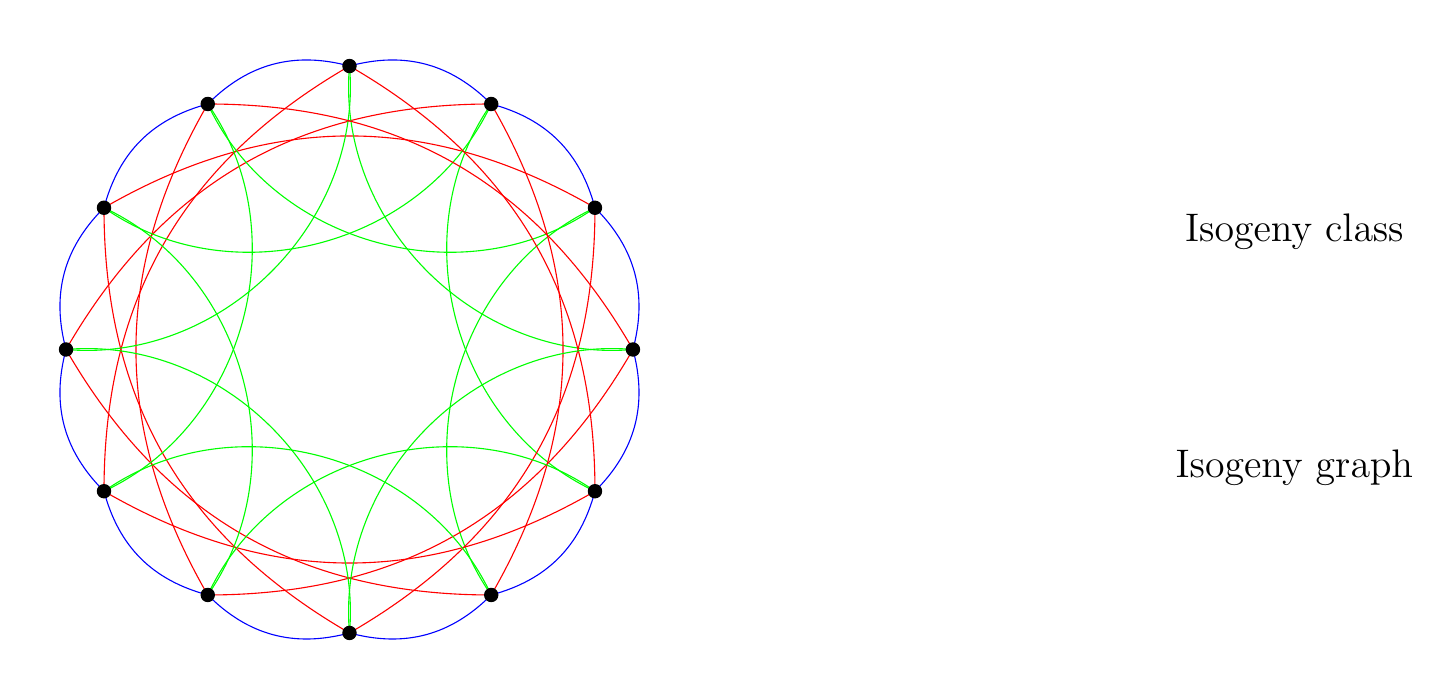
\begin{tikzpicture}
    \begin{scope}[scale=1.2]
      \def\crater{12}
      \def\jumpa{-8}
      \def\jumpb{9}
      \def\diam{3cm}

      \uncover<2->{
        \foreach \i in {1,...,\crater} {
          \draw[blue] (360/\crater*\i : \diam) to[bend right] (360/\crater*\i+360/\crater : \diam);
          \draw[red] (360/\crater*\i : \diam) to[bend right] (360/\crater*\i+\jumpa*360/\crater : \diam);
          \draw[green] (360/\crater*\i : \diam) to[bend right=50] (360/\crater*\i+\jumpb*360/\crater : \diam);
        }
      }
      \foreach \i in {1,...,\crater} {
        \draw[fill] (360/\crater*\i: \diam) circle (2pt) +(360/\crater*\i: 0.4);
      }
    \end{scope}

    \begin{scope}
      \Large
      \uncover<1->{\node at (12,1.5) {Isogeny class};}
      \uncover<2->{\node at (12,-1.5) {Isogeny graph};}
    \end{scope}
  \end{tikzpicture}
\end{frame}

%%

\begin{frame}{The isogeny problem}
  \Large\centering
  \begin{tikzpicture}[scale=2]
    \node (E) at (0,0) {$E$};
    \node (E1) at (8,0) {$E'$};
    \uncover<2->{
      \draw[-latex] (E) edge node[above] {??} (E1);
    }
  \end{tikzpicture}
\end{frame}

%%

\begin{frame}{Isogeny Yantras}
  \centering\large
  \begin{tikzpicture}
    \begin{scope}
      \draw (0:0) node(A){$E$};
      \foreach  \i in {0,...,7} {
        \draw[-latex] (A) edge (90/7*\i-45:2);
      }
    \end{scope}
    
    \begin{scope}[xshift=8cm]
      \fill (0,0) node(A){$E$} (4,0) node(B){$E'$};
      \foreach  \i in {-4,...,4} {
        \draw[-latex] (A) edge[bend left=\i*20] (B);
      }
      \node at (2,-3) {$\Hom(E,E')$};
      \node at (2,-4) {\emph{Ideal class}};
    \end{scope}
    
    \begin{scope}[xshift=20cm]
      \fill (0,-1) node(A){$E$};
      \foreach  \i in {1,...,8} {
        \draw[-latex] (A) edge[loop,out=90+10*\i,in=90-10*\i,looseness=20-\i] (A);
      }
      \node at (0,-3) {$\End(E)$};
      \node at (0,-4) {\emph{Order}};
    \end{scope}
  \end{tikzpicture}
\end{frame}

%%

\begin{frame}{Degree}
  \begin{columns}
    \large
    \begin{column}{0.5\textwidth}
      \centering
      \[\deg(φ) ∈ ℕ^+\]

      \begin{itemize}
      \item A measure of ``size'';
      \item<2-> \emph{Multiplicative;}
      \end{itemize}
    \end{column}
    \begin{column}{0.5\textwidth}
      \centering
      \begin{tikzpicture}
        \fill
        (0,0) circle (1mm) node(A){}
        ++(3,0) circle (1mm) node(B){}
        ++(6,0) circle (1mm) node(C){};
        \draw[-latex]
        (A) edge[bend left] node[above]{$φ$} (B)
        (B) edge[bend left] node[above]{$ψ$} (C);

        \uncover<2->{
          \node at (4.5,-2) {\emph{$\deg(ψ∘φ) = \deg(ψ)\deg(φ)$}};
        }
      \end{tikzpicture}
    \end{column}
  \end{columns}
\end{frame}

%%

\begin{frame}{The larger the degree, the more isogenies}
  \centering\Large
  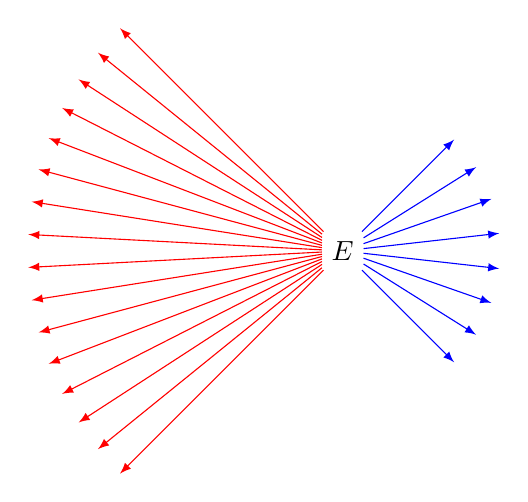
\begin{tikzpicture}
    \draw (0:0) node(A){$E$};
    \foreach  \i in {0,...,7} {
      \draw[blue,-latex] (A) edge (90/7*\i-45:2);
    }
    \foreach  \i in {0,...,15} {
      \draw[red,-latex] (A) edge (90/15*\i-45:-4);
    }
  \end{tikzpicture}
\end{frame}

%%

\begin{frame}{Degree}
  \begin{columns}
    \large
    \begin{column}{0.5\textwidth}
      \centering
      \[\deg(φ) ∈ ℕ^+\]

      \begin{itemize}
      \item A measure of ``size'';
      \item \emph{Multiplicative;}
      \item A measure of ``complexity'':\\
        only isogenies of small degree fit into a computer!
      \end{itemize}
    \end{column}
    \begin{column}{0.5\textwidth}
      \centering
      \begin{tikzpicture}
        \fill
        (0,0) circle (1mm) node(A){}
        ++(3,0) circle (1mm) node(B){}
        ++(6,0) circle (1mm) node(C){};
        \draw[-latex]
        (A) edge[bend left] node[above]{$φ$} (B)
        (B) edge[bend left] node[above]{$ψ$} (C);

        \node at (4.5,-2) {\emph{$\deg(ψ∘φ) = \deg(ψ)\deg(φ)$}};
      \end{tikzpicture}
    \end{column}
  \end{columns}
\end{frame}

%%

\begin{frame}{Isogenies of smooth degree}
  \Large
  \begin{columns}
    \begin{column}{0.45\textwidth}
      \centering
      degree
      \only<1>{$2$}%
      \only<2>{$4$}%
      \only<3>{$8$}%
      \only<4>{$16$}%
      \only<5>{$2^x$}
    \end{column}
    \begin{column}{0.55\textwidth}
      \centering
      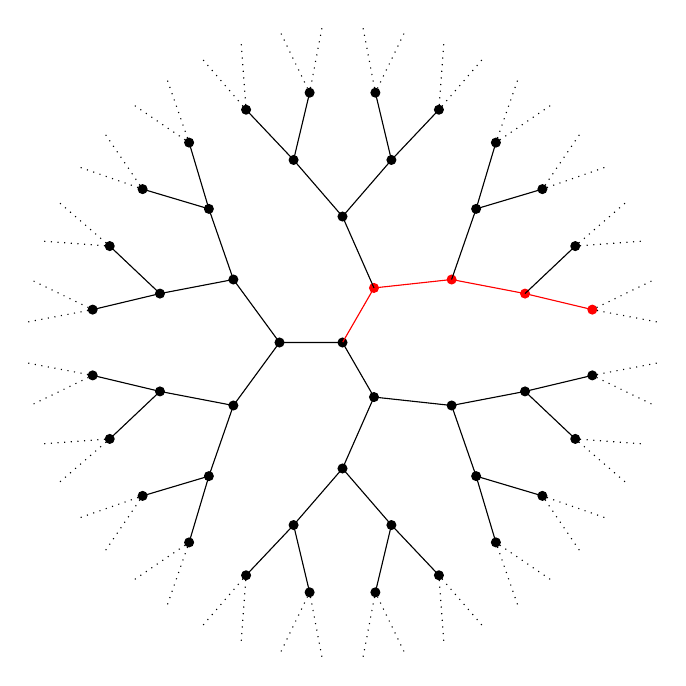
\begin{tikzpicture}[scale=0.8]
        \def\levels{5}
        \draw[fill] (0:0) circle (2pt);
        \foreach \i in {1,...,\levels} {
          \pgfmathparse{3*2^\i}
          \let\nodes\pgfmathresult
          \foreach \j in {1,3,...,\nodes} {
            \pgfmathparse{\j + (-1)^div(\j,2)}
            \let\lower\pgfmathresult
            \uncover<\i->{
              \ifthenelse{\i = \levels}{
                \draw[dotted] (360/\nodes*\j : \i) --
                (360/\nodes*\lower : \i - 1);
              }{
                \pgfextra{
                  \ifthenelse{\j=1}{\def\col{red}}{\def\col{black}}
                  \draw[fill,\col] (360/\nodes*\j : \i) circle (2pt) --
                  (360/\nodes*\lower : \i - 1);
                }
              }
            }
          }
        }
      \end{tikzpicture}
    \end{column}
  \end{columns}
\end{frame}

%%

\begin{frame}{Key exchange?}
  \large\centering
  \begin{tikzpicture}
    \fill
    (0,0) circle (1mm) node(O){}
    (8,3) circle (1mm) node(A){}
    (8,-3) circle (1mm) node(B){}
    (16,0) circle (1mm) node(S){};
    \draw[-latex]
    (O) edge node[above]{$\mathrm{sk}_A$} (A)
    edge  node[below]{$\mathrm{sk}_B$} (B)
    (A) edge node[above]{??} (S)
    (B) edge node[below]{??} (S);
  \end{tikzpicture}
\end{frame}

%%

\begin{frame}{Push-forward}
  \large\centering
  \begin{tikzpicture}
    \node at (21,2) {$\bigl(\deg(φ), \deg(ψ)\bigr) = 1$};
    
    \fill
    (0,0) circle (1mm) node(O){}
    (8,3) circle (1mm) node(A){}
    (8,-3) circle (1mm) node(B){};
    \draw[-latex]
    (O) edge node[above] {$φ$} (A)
     edge node[below] {$ψ$} (B);
    
    \uncover<6->{\fill (16,0) circle (1mm) node(S){};}
    \foreach \i in {2,...,5} {
      \uncover<\i>{
        \draw[dashed,-latex] ($(O)!\i/5-1/5!(A)$) to ($(B)!\i/5-1/5!(S)$);
      }
    }
    \uncover<6->{
      \draw[-latex] (A) edge node[above] {$φ_*ψ$} (S);
      \node at (21,0) {$\deg(φ_*ψ) = \deg(ψ)$};
    }

    \foreach \i in {7,...,10} {
      \uncover<\i>{
        \draw[dashed,-latex] ($(O)!\i/5-6/5!(B)$) to ($(A)!\i/5-6/5!(S)$);
      }
    }
    \uncover<11->{
      \draw[-latex] (B) edge node[below] {$ψ_*φ$} (S);
      \node at (21,-2) {$\deg(ψ_*φ) = \deg(φ)$};
    }
  \end{tikzpicture}  
\end{frame}

%%

\begin{frame}{Supersingular Isogeny Diffie-Hellman (SIDH)}
  \large\centering
  \begin{tikzpicture}
    \fill
    (0,0) circle (1mm) node(O){}
    (0,-6) circle(1mm) node(B){};

    \draw[-latex,red]
    (O) edge node[right] {$ψ_0$} (-45:6)
    edge node[left] {$ψ_n$} (-135:6);
    \draw[-latex] (O) edge node[left] {$ψ_{B}$} (B);
    \draw (-45:1) arc (-45:-90:1) node[midway,below] {$\mathrm{sk}_B$};

    \begin{scope}[xshift=20cm]
      \uncover<2->{
        \fill (0,0) circle (1mm) node(A){};
        \draw[-latex] (O) edge node[above]{$φ_{A}$} (A);
        \draw[-latex,red]
        (A) edge node[right] {$φ_{A*}ψ_0$} (-45:6)
        edge node[left] {$φ_{A*}ψ_n$} (-135:6);
      }

      \uncover<3->{
        \fill (0,-6) circle (1mm) node(S){};
        \draw[-latex] (A) edge (S);
        \draw (-45:1) arc (-45:-90:1) node[midway,below] {$\mathrm{sk}_B$};
      }
    \end{scope}

    \uncover<4->{
      \draw[-latex] (B) edge (S);
    }
  \end{tikzpicture}
\end{frame}

%%

\begin{frame}{The Deuring Correspondence}
  \large\centering
  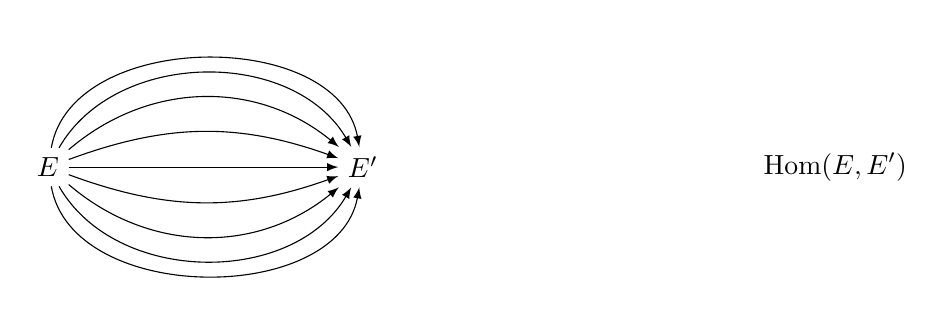
\begin{tikzpicture}
    \fill (0,0) node(A){$E$} (4,0) node(B){$E'$};
    \foreach  \i in {-4,...,4} {
      \draw[-latex] (A) edge[bend left=\i*20] (B);
    }
    \node at (10,0) {$\Hom(E,E')$};
  \end{tikzpicture}
\end{frame}

%%

\begin{frame}[plain]
  \centering
  
\includegraphics[height=\textheight]{om.png}
\end{frame}

%%

\begin{frame}{Homs are groups}
  \large\centering
  \begin{tikzpicture}
    \node (E1) at (0,0) {$E'$};
    \node (E) at (10,0) {$E$};
    \uncover<2->{
      \draw[dashed,->] (E) edge node[above] {$φ+ψ$} (E1);
    }
    
    \draw[->] (E) edge[bend right] node[above] {$φ$} (E1)
    edge[bend left] node[below] {$ψ$} (E1);

    \begin{scope}[xshift=20cm]
      \node at (0,1) {$φ,ψ ∈ \Hom(E,E')$};

      \uncover<2->{
        \node at (0,-1) {$(φ + ψ)(P) := φ(P) + ψ(P)$};
      }
    \end{scope}
  \end{tikzpicture}
\end{frame}

%%

\begin{frame}{Ends are rings}
  \large
  \begin{columns}
    \begin{column}{0.5\textwidth}
      \centering
      Distributivity
    \end{column}
    \begin{column}{0.5\textwidth}
      \centering
      \begin{align*}
        φ∘(ψ+χ) &= (φ∘ψ)+(φ∘χ)\\[2em]
        (ψ+χ)∘φ &= (ψ∘φ)+(χ∘φ)\\
      \end{align*}      
    \end{column}
  \end{columns}
\end{frame}

%%

\begin{frame}{Supersingular endomorphism rings}
  \centering\large
  \begin{tikzpicture}
    {\Large
      \draw
      (0,0) node(End){$\End(E)$}
      (3,0) node{$≃$}
      (6,0) node(O){$\O$}
      (9,0) node{$⊂$}
      (12,0) node(B){$\mathcal{B}_{p,∞}$};
    }

    \uncover<2->{\draw[->] (14,-2) node(X){quaternion algebra} (X) to (B);}
    \uncover<3->{\draw[->] (0,-2) node(X) {maximal order} (X) to (O);}
    \uncover<4->{
      \draw
      (14,-3) node {4-dimensional $ℚ$-vector space}
      (0,-3) node {rank 4 submodule};
    }
  \end{tikzpicture}

  \vspace{1.5cm}

  \uncover<5->{ \emph{EndRing problem:} given $E$ supersingular,
    compute an order $\O ≃ \End(E)$.  }
\end{frame}

%%

\begin{frame}{Homs $\longleftrightarrow$ Modules  $\longleftrightarrow$ Ideals}
  \large\centering
  \begin{tikzpicture}
    \begin{scope}
      \node (E1) at (0,0) {$E'$};
      \node (E) at (6,0) {$E$};

      \draw[-latex] (E) edge node[above] {$φ$} (E1);
      \uncover<1,4->{
        \node at (3,-3) {$φ ∈ \Hom(E,E')$};
      }

      \uncover<2>{
        \draw[-latex] (E) edge[loop,out=45,in=-45,looseness=10] node[right] {$ω$} (E);
        \node at (3,-3) {$φ∘ω ∈ \Hom(E,E')$};
      }
      
      \uncover<3>{
        \draw[-latex] (E1) edge[loop,out=135,in=225,looseness=10] node[left] {$ω'$} (E1);
        \node at (3,-3) {$ω'∘φ ∈ \Hom(E,E')$};
      }
    \end{scope}

    \uncover<4->{
      \begin{scope}[xshift=15cm]
        \node (O) at (0,0) {$\O$};
        \node (O1) at (6,0) {$\O'$};
        \draw[-latex] (O) edge node[above] {$I_φ$} (O1);
        
        \node at (3,-2.5) {$\Hom(E,E') ≃ I_φ$};
        \node at (3,-3.5) {$\O ⊃ I_φ ⊂ \O'$};
      \end{scope}
    }
  \end{tikzpicture}
\end{frame}

%%

\begin{frame}
  \Large
  \begin{tikzpicture}[remember picture,overlay,shift={(current page.center)}]
    \fill[white] (0,8) -- (16,8) -- (16,-8) -- (0,-8);
    \fill[ibmblue] (0,8) -- (-16,8) -- (-16,-8) -- (0,-8);

    \draw[ibmblue]
    (8,3) node {Maximal order}
    ++(0,-2) node {Ideal}
    ++(0,-2) node {Ideal class}
    ++(0,-2) node {Norm};
    \draw[white]
    (-8,3) node {Endomorphism ring}
    ++(0,-2) node {Isogeny}
    ++(0,-2) node {$\Hom(E,E')$}
    ++(0,-2) node {Degree};

  \end{tikzpicture}
\end{frame}

%%

\begin{frame}{Kohel-Lauter-Petit-Tignol (KLPT)}
  \Large\centering
  \begin{tikzpicture}[scale=2]
    \node (E) at (0,0) {\alt<1>{$E$}{$\End(E)$}};
    \node (E1) at (8,0) {\alt<1>{$E'$}{$\End(E')$}};
    \draw[-latex] (E) edge node[above] {\alt<1-2>{??}{$I$}} (E1);
    \uncover<3->{\node at (4,-1) {$N(I) = 2^x$};}
  \end{tikzpicture}

  \vspace{1.5cm}

  \uncover<4->{
    \emph{Corollary:}~~~~ Isogeny problem $\quad≃\quad$ EndRing problem
  }
\end{frame}

%% 

\begin{frame}{Contagious knowledge}
  \centering
  \begin{tikzpicture}
    \pgfmathsetseed{1}
    \foreach \i in {1,...,200} {
      \pgfmathparse{30*random()}
      \let\x\pgfmathresult
      \pgfmathparse{7*random()}
      \let\y\pgfmathresult
      \fill[black!20!white] (\x,\y) circle (1pt);
    }
    \foreach \i in {1,...,10} {
      \pgfmathparse{28*random()}
      \let\x\pgfmathresult
      \pgfmathparse{6*random()}
      \let\y\pgfmathresult
      \fill (\x,\y) circle (2pt);
      \uncover<2->{
        \foreach \rho in {0,1,2} {
          \draw[fill,-latex] (\x,\y) -- +(120*\rho:.3) circle (2pt);
          \uncover<3->{
            \foreach \sigma in {-1,1} {
              \draw[fill,-latex] (\x,\y) ++(120*\rho:.3) -- ++(120*\rho+60*\sigma:.3) circle (2pt);
            }
          }
        }
      }
    }
  \end{tikzpicture}
\end{frame}

%%

\begin{frame}{SQIsign \small(identification scheme)}
  \transdissolve<4,6>
  \large
  \centering
  \begin{tikzpicture}[very thick]
    \fill
    (0,4) node(E0){} circle (4pt);
    \draw
    (-8,0) node(PK){} circle (4pt);
    \draw[dashed,->>>>] (PK) edge node[above,sloped] {secret key} (E0);
    
    \uncover<2->{
      \draw (12,4) node(COM){} circle (4pt);
      \draw[dashed,->>>>] (E0) edge node[sloped,above] {commitment} (COM);
    }

    \uncover<3->{
      \draw (20,0) node(CH){} circle (4pt);
    }
    \uncover<3,6->{
      \draw (COM) edge[->] node[sloped,above] {challenge} (CH);
    }

    \uncover<4-5>{
      \draw (COM) edge[dashed,->>>>] node[sloped,above] {challenge} (CH);
    }

    \uncover<5>{
      \draw (PK) edge[dashed,->>>>] (CH);
    }

    \uncover<6->{
      \node at (6,1.5) {\includegraphics[height=2cm]{wizard-hat}};
      \node at (6.7,0.8) {\small KLPT};
      \draw (PK) edge[->] node[below] {response} (CH);
    }
  \end{tikzpicture}
\end{frame}

%%

\begin{frame}{SQIsign}
  \large
  \begin{table}[h]
    \centering
    \begin{tabular}{ r r | r r r | c }
      \multicolumn{2}{c|}{Bytes} & \multicolumn{3}{c|}{Mcycles}\\
       Public Key & Signature & Keygen & Sign & Verify & Security \\
      \hline
       64 & 177 & 3,728 & 5,779 & 108 & NIST-1 \\
       96 & 263 & 23,734 & 43,760 & 654 & NIST-3 \\
       128 & 335 & 91,049 & 158,544 & 2,177 & NIST-5 \\
    \end{tabular}
  \end{table}
\end{frame}

%%

\begin{frame}{Higher dimensional abelian varieties}
  \centering
  \begin{tikzpicture}[domain=-2.4566:4,samples=100]
    \begin{scope}[xscale=0.3,yscale=0.5]
      \draw plot (\x,{sqrt(\x*\x*\x-4*\x+5)});
      \draw plot (\x,{-sqrt(\x*\x*\x-4*\x+5)});
      \node (P1) at (3,4.47213595499958) {};
    \end{scope}
    \begin{uncoverenv}<2->
      \begin{scope}[xscale=0.7,yscale=0.15,shift={(7,-20)}]
        \draw plot ({sqrt(\x*\x*\x-4*\x+5)},\x);
        \draw plot ({-sqrt(\x*\x*\x-4*\x+5)},\x);
        \node (P2) at (-4.47213595499958,3) {};
      \end{scope}
      \node at (5,0) {\huge $E×E$};
      
      \fill (P1) circle (2pt);
      \fill (P2) circle (2pt);

      \draw[dashed] (P2) -- (P2 |-, |- P1) -- (P1);
      \fill (P2 |-, |- P1) circle (2pt) node[above right] {$(P,Q)$};
    \end{uncoverenv}
  \end{tikzpicture}
\end{frame}

%%

\begin{frame}{Higher dimensional isogenies}
  \large
  \begin{columns}
    \begin{column}{0.4\textwidth}
      \centering
      \begin{tikzpicture}[scale=2]
        \uncover<2->{
          \node (A) at (-1,1) {$A$};
          \node (B) at (1,-1) {$B$};
          \node (C) at (1,1) {$C$};
          \node (D) at (-1,-1) {$D$};
          
          \draw[-latex] (A) edge node[above] {$α$} (C) edge node[left] {$β$} (D)
          (B) edge node[right] {$γ$} (C) edge node[below] {$δ$} (D);
        }
      \end{tikzpicture}
    \end{column}
    \begin{column}{0.6\textwidth}
      \begin{align*}
        A × B &→ C × D\\
        \uncover<2->{(P,Q) &↦ \bigl( α(P) + γ(Q), β(P) + δ(Q) \bigr)}\\
              &\uncover<3->{=
                \begin{pmatrix}
                  α&γ\\β&δ
                \end{pmatrix}
                \begin{pmatrix}
                  P\\Q
                \end{pmatrix}}
      \end{align*}
    \end{column}
  \end{columns}
\end{frame}

%%

\begin{frame}{Isogeny problem + Torsion point information (SIDH)}
  \large\centering
  \begin{tikzpicture}
    \fill
    (0,0) circle (1mm) node(O){};

    \draw[-latex,red]
    (O) edge node[right] {$ψ_0$} (-45:6)
    edge node[left] {$ψ_n$} (-135:6);

    \begin{scope}[xshift=20cm]
      \fill (0,0) circle (1mm) node(A){};
      \draw[dashed,-latex] (O) edge node[above]{$φ_{A}$} (A);
      \draw[-latex,red]
      (A) edge node[right] {$φ_{A*}ψ_0$} (-45:6)
      edge node[left] {$φ_{A*}ψ_n$} (-135:6);
    \end{scope}
  \end{tikzpicture}
\end{frame}

%%

\begin{frame}
  \large\centering
  \begin{tikzpicture}
    \begin{scope}[domain=-2.4566:4,samples=100,scale=0.6]
      \begin{scope}[xscale=0.3,yscale=0.5]
        \draw plot (\x,{sqrt(\x*\x*\x-4*\x+5)});
        \draw plot (\x,{-sqrt(\x*\x*\x-4*\x+5)});
        \node (P1) at (3,4.47213595499958) {};
      \end{scope}
      \begin{scope}[xscale=0.7,yscale=0.15,shift={(7,-20)}]
        \draw plot ({sqrt(\x*\x*\x-4*\x+5)},\x);
        \draw plot ({-sqrt(\x*\x*\x-4*\x+5)},\x);
        \node (P2) at (-4.47213595499958,3) {};
      \end{scope}
    \end{scope}

    \draw[-latex] (7,0) to node[above]{$Φ_A$} (17,0);
    \node at (12,-2) {$\deg(φ_A) ≈ \deg(Φ_A) = 2^x$};
    
    \begin{scope}[domain=-2.4566:4,samples=100,xshift=19cm,scale=0.6]
      \begin{scope}[xscale=0.3,yscale=0.5]
        \draw plot (\x,{sqrt(\x*\x*\x-4*\x+5)});
        \draw plot (\x,{-sqrt(\x*\x*\x-4*\x+5)});
        \node (P1) at (3,4.47213595499958) {};
      \end{scope}
      \begin{scope}[xscale=0.7,yscale=0.15,shift={(7,-20)}]
        \draw plot ({sqrt(\x*\x*\x-4*\x+5)},\x);
        \draw plot ({-sqrt(\x*\x*\x-4*\x+5)},\x);
        \node (P2) at (-4.47213595499958,3) {};
      \end{scope}
    \end{scope}
  \end{tikzpicture}
\end{frame}

%%

\begin{frame}{SQIsign2D}
  \transdissolve<4,6>
  \large
  \centering
  \begin{tikzpicture}[very thick]
    \fill (0,4) node(E0){} circle (4pt);
    \draw (8,4) node(PK){} circle (4pt);
    \draw (E0) edge[double distance=2pt,dashed,-{Implies[] Implies[] Implies[] Implies[]}] node[above,sloped] {secret key} (PK);
    
    \uncover<2->{
      \draw (-1,0) node(COM){} circle (4pt);
      \draw (COM) edge[double distance=2pt,dashed,-{Implies[] Implies[] Implies[] Implies[]}] node[sloped,above] {commitment} (E0);
    }

    \uncover<3->{
      \draw (9,0) node(CH){} circle (4pt);
    }
    \uncover<3,6->{
      \draw (PK) edge[->] node[sloped,above] {challenge} (CH);
    }

    \uncover<4-5>{
      \draw (PK) edge[double distance=2pt,dashed,-{Implies[] Implies[] Implies[] Implies[]}] node[sloped,above] {challenge} (CH);
    }

    \uncover<5>{
      \draw (COM) edge[double distance=2pt,dashed,-{Implies[] Implies[] Implies[] Implies[]}] (CH);
    }

    \uncover<6->{
      \node at (4,1.5) {\includegraphics[height=2cm]{wizard-hat}};
      \node at (5,0.8) {\small LLL + HD};
      \draw (COM) edge[double distance=2pt,-Implies] node[below] {response} (CH);
    }
  \end{tikzpicture}
\end{frame}

%% 

\begin{frame}{SQIsign2D}
  \large
  \begin{table}[h]
    \centering
    \begin{tabular}{ r r | r r r | c }
      \multicolumn{2}{c|}{Bytes} & \multicolumn{3}{c|}{Mcycles}\\
      Public Key & Signature & Keygen & Sign & Verify & Security \\
      \hline
      66 & 148 & 60 & 160 & 9 & NIST-1 \\
      98 & 222 & 170 & 460 & 29 & NIST-3 \\
      130 & 294 & 360 & 940 & 62 & NIST-5 \\
    \end{tabular}
  \end{table}
\end{frame}

%%

\begin{frame}[plain]
  \begin{tikzpicture}[remember picture,overlay,shift={(current page.center)}]
    \begin{scope}[scale=4,rotate=180]
      \fill[white] (0,2) -- (-4,2) -- (-4,-2) -- (0,-2);
      \fill (0,2) -- (4,2) -- (4,-2) -- (0,-2);
    
      % color one half of a unit circle
      \begin{scope}
        \fill[white] (0,0) circle (1cm);
        \clip (0,0) circle (1cm);
        \fill[black] (0cm,1cm) rectangle (-1cm, -1cm);
      \end{scope}
      
      % fill heads
      \fill[black] (0,0.5) circle (0.5cm);
      \fill[white] (0,-0.5) circle (0.5cm);

      % fill eyes
      \fill[white] (0,0.5) circle (0.15cm);
      \fill[black] (0,-0.5) circle (0.15cm);

      % fill outside
      \fill[black] (0,1.5) circle (0.5cm);
      \fill[white] (0,-1.5) circle (0.5cm);
    \end{scope}

    \node[white] at (-9.5,0) {\Huge CRYPTANALYSIS};
    \node at (9.5,0) {\Huge CRYPTOGRAPHY};
    
  \end{tikzpicture}
\end{frame}

\end{document}


% LocalWords:  Isogeny abelian isogenies hyperelliptic supersingular Frobenius
% LocalWords:  isogenous
